
\begin{figure}
	\centering
	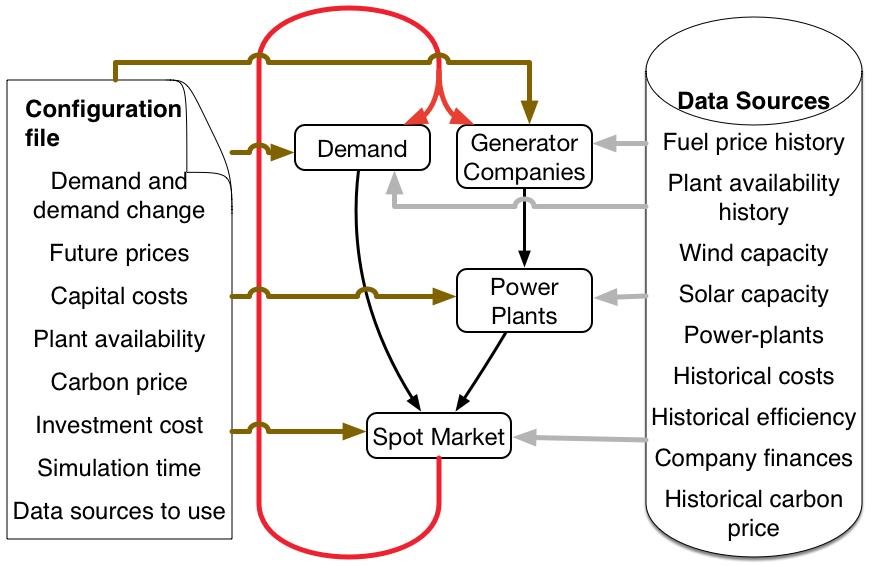
\includegraphics[width=0.85\linewidth]{figures/System_overview_large.png}
	\caption{High level overview.}
	\label{fig:systemoverview}
	\vskip -6.9mm
\end{figure}

\begin{figure*}
	\centering
	\includegraphics[width=0.8\linewidth]{figures/low_level_system}
	\caption{ElecSim simulation overview}
	\label{fig:lowlevelsystem}
\end{figure*}

ElecSim is made up of five fundamental parts: the agents, which are split up into demand and GenCos; power plants; a Power Exchange, which controls an electricity spot market; and the data for parametrisation. A schematic of ElecSim is displayed in Figure \ref{fig:systemoverview}.

\textit{Data parametrisation.} ElecSim contains a configuration file and a collection of data sources for parametrisation. These data sources contain information such as historical fuel prices, historical plant availability, wind and solar capacity.

The configuration file allows for rapid changes to test different hypothesis and scenarios, and points to the different data sources. The configuration file enables one to change the demand growth and shape, future fuel and carbon prices, capital costs, plant availability, investment costs and simulation time.

\textit{Demand Agent.} The demand agent is a simplified representation of aggregated demand in a country. The demand is represented as a load duration curve (LDC). \vphantom{\color{red}An example load duration curve for a year is demonstrated in Figure \ref{fig:loaddurationcurve}.} An LDC is an arrangement of all load levels in descending order of magnitude. \vphantom{\color{red}, where the lowest segment demand demonstrates baseload, and the highest segment represents peak demand.} Each year, the demand agent changes each of the LDC segments proportionally.

% \begin{figure}
% 	\centering
% 	\includegraphics[width=0.95\linewidth]{figures/load_duration_curve}
% 	\caption{{\color{red}Example load duration curve in a single year.}}
%  	\label{fig:loaddurationcurve}
% \end{figure}

As per Chappin \textit{et al.} \cite{Chappin2017}, we modelled the LDC of electricity demand with twenty segments. Twenty segments enabled us to capture the variation in demand throughout the year to a high degree of accuracy, whilst reducing computational complexity. 


\textit{Generation Company Agents.} The GenCos have two main functions. Investing in power plants and making bids to sell their generation capacity. We will first focus on the buying and selling of electricity, and then cover the investment algorithm.

The power exchange runs every year, accepting the lowest bids until supply meets demand. Once this condition is met, the spot price or system marginal price (SMP) is paid to all generators regardless of their initial bid. Generators are motivated to bid their SRMC, to ensure that their generator is being utilised, and reduce the risk of overbidding.

\textit{Investment.} Investment in power plants is made based upon a net present value (NPV) calculation. NPV is a summation of the present value of a series of present and future cash flow. NPV provides a method for evaluating and comparing investments with cash flows spread over many years, making it suited for evaluating power plants which have a long lifetime.  \vphantom{\color{red}NPV is based upon the fact that current cash flow is worth more than future cash flow. This is due to the fact that money today can be invested and have a rate of return. This means that, for example \$50,000 today is worth more than \$50,000 in 10 years time. The value in which future cash flow is worth less than present cash flow is discounted by the discount rate.}

Equation \ref{eq:npv_eq} is the calculation of NPV, where $t$ is the year of the cash flow, $i$ is the discount rate, $N$ is total number of periods, or lifetime of power plant, and $R_t$ is the net cash flow at time $t$.
\begin{equation} \label{eq:npv_eq}
NPV(i, N) = \sum_{t=0}^{N}\frac{R_t}{(1+t)^t}
\end{equation}
A discount rate set by a GenCo's weighted average cost of capital (WACC) is often used \cite{KincheloeStephenC1990TWAC}. WACC is the rate that a company is expected to pay on average for its stock and debt. Therefore to achieve a positive NPV, an income larger than the WACC is required. However, a higher WACC is often selected to adjust for varying risk profiles, opportunity costs and rates of return. To account for these differences we sample from a Gaussian distribution, giving us sufficient variance whilst deviating from the expected price.

To calculate the NPV, future market conditions must be considered. For this, each GenCo forecasts $N$ years into the future, which we assume is representative of the lifetime of the plant. As in the real world, GenCos have imperfect information, and therefore must forecast expected demand, fuel prices, carbon price and electricity sale price. This is achieved by fitting functions to historical data. Each GenCo is different in that they will use differing historical time periods of data for forecasting.

Fuel and carbon price are forecast using linear regression. Demand, however, is forecast using an exponential function, which considers compounded growth. Linear regression is used if an exponential function is found to be sub-optimal.

This forecasted data is then used to simulate a market $N$ years into the future using the electricity market algorithm. We simulate a market based on the expected bids -- based on SRMC -- that every operating power plant will make. This includes the removal of plants that will be past their operating period, and the introduction of plants that are in construction or pre-development stages. 

There may be scenarios where demand is forecast to grow significantly, and limited investments have yet been made to meet that demand. The expected price, would be that of lost load. Lost load is defined as the price customers would be willing to pay to avoid disruption in their electricity supply. To avoid GenCos from estimating large profits, and under the assumption that further power plant investments will be made, the lost load price is replaced with a predicted electricity price using linear regression based on prices at lower points of the demand curve. If zero segments of demand are met, then the  lost load price is used to encourage investment. 

Once this data has been forecasted\vphantom{Once expected fuel prices, carbon price, discount rate, and expected sale price of electricity are all forecast}, the NPV can be calculated. GenCos must typically provide a certain percentage of upfront capital, with the rest coming from investors in the form of stock and shares or debt (WACC). The percentage of upfront capital can be customised by the user in the configuration file. The GenCos then invest in the power plants with the highest NPV. 


\textit{Power Plant Parameters.}\label{ssssec:powerplantparameters} Costs form an important element of markets and investment, and publicly available data for power plant costs for individual countries can be scarce. Thus, extrapolation and interpolation is required to estimate costs for power plants of differing sizes, types and years of construction.

Users are able to initialise costs relevant to their particular country by providing detailed cost parameters. They can also provide an average cost per MWh produced over the lifetime of a plant, known as levelised cost of electricity (LCOE).

The parameters used to initialise the power plants are detailed in this section. Periods have units of years and costs in \textsterling/MW unless otherwise stated: Efficiency ($\eta$) is defined as the percentage of energy from fuel that is converted into electrical energy (\%). Operating period ($OP$) is the total period in which a power plant is in operation. Pre-development period ($P_D$) and pre-development costs ($P_C$) include the time and costs for pre-licensing, technical and design, as well as costs incurred due to regulatory, licensing and public enquiry. The construction period ($C_D$) and construction costs ($C_C$) are incurred during the development of the plant, excluding network connections. The infrastructure costs ($I_C$) are the costs incurred by the developer in connecting the plant to the electricity or gas grid (\textsterling). Fixed operation \& maintenance costs ($F_C$) are costs incurred in operating the plant that do not vary based on output. Variable operation \& maintenance ($V_C$) costs are incurred in operating the plant that depend on generator output \cite{Ltd2016}.



%\begin{table}[h]
%	\centering
%	\csvautobooktabular{tables/notation_formated.csv}
%	\caption{Parameter notation. (Whilst the unit of currency displayed is \textsterling, this can be modified to other currencies eg. \$, \texteuro)}
%	\label{table:parameter_notation}
%\end{table}
%\addtolength{\textfloatsep}{-0.2in}

Precise data is not available for every plant size. Linear interpolation is used to estimate individual prices between known points. When the plant to be estimated falls outside of the range of known data points, the closest power plant is used. We experimented with extrapolation but this would often lead to unrealistic costs. %{\color{red}For example, the parameters of a 1,500MW combined cycle gas plant (CCGT) are estimated to be the same as a 1,200MW CCGT plant if the 1,200MW plant was the largest available data point. }

If specific parameters are not known, then the LCOE can be used for parameter estimation, through the use of linear optimisation. Constraints can be set by the user, enabling, for example, varying operation and maintenance costs per country as a fraction of LCOE.

To fully parametrise power plants, availability and capacity factors are required. Availability is the percentage of time that a power plant can produce electricity. This can be reduced by forced or planned outages. We integrate historical data to model improvements in reliability over time.

The capacity factor is the actual electrical energy produced over a given time period divided by the maximum possible electrical energy it could have produced. The capacity factor can be impacted by regulatory constraints, market forces and resource availability. For example, higher capacity factors are common for photovoltaics in the summer, and lower in winter. 

To model the intermittency of wind and solar power we allow them to contribute only a certain percentage of their total capacity (nameplate capacity) for each load segment. This percentage is based upon empirical wind and solar capacity factors. In this calculation we consider the correlation between demand and renewable resources. We are unable to model short-term storage due to ElecSim taking a single time-step per year. 

When initialised, $V_C$ is selected from a uniform distribution, with the ability for the user to set maximum percentage increase or decrease. A uniform distribution was chosen to capture the large deviations that can occur in $V_C$, especially over a long time period. \vphantom{By doing this, the variance in costs between individual power plants for processes such as preventative and corrective maintenance, labour costs and skill, health and safety and chance are different per plant instant.}

Fuel price is controlled by the user, however, there is inherent volatility in fuel price. To take into account this variability, an ARIMA \cite{ARIMA} model was fit to historical gas and coal price data. The standard deviation of the residuals was used to model the variance in price that a GenCo will buy fuel in a given year. This considers differences in chance and hedging strategies.


%\vphantom{With historical power plants which have been refurbished, we sample their initialisation randomly between 15 years prior to the initialisation year and the initialisation year. This is done because there is rarely a comprehensive data set on when plants are refurbished. 15 years was chosen due to the fact that plants often have an operating period of 25 years, and therefore 15 years allowed for sufficient variance in results, whilst keeping plants in operation.}

Figure \ref{fig:lowlevelsystem} demonstrates the simulation and how it co-ordinates runs. The world contains data and brings together GenCos, the Power Exchange and demand. The investment decisions are based on future demand and costs, which in turn influence bids made.

Exogenous variables include fuel and \ce{CO2} prices as well as demand growth. Once the data is initialised, the world calls on the Power Exchange to operate the yearly electricity spot market. The world also settles the accounts of the GenCos, by paying bids, and removing operating and capital costs as well as loans and dividends.

%The world contains the functionality to dismantle old plants once they have reached the end of their lifetime. Power plants are taken out of service if they have not sold any electricity in the past 7 years, which is configurable in the configuration file. We decided upon this due to the fact that power generators have high, sunk capital costs, which often have high demolition costs. We assume, therefore, that generator companies are willing to wait circa $\frac{1}{4}$ of their lives to see if a pay-out occurs due to the breakdown of competing power plants, increasing demand, or governmental support in the form of a carbon tax increase or reduction.






%GenCos  invest in power plants based on the highest positive net present value (NPV). Bids are made for each power plant based on the power plants short run marginal cost. A Power Exchange operator matches these bids with demand in merit order. 



%\begin{figure}[h]
%	\begin{center}
%		\includegraphics[width=0.5\textwidth]{figures/System_overview.pdf}
%		\caption{ElecSim simulation overview.}
%		\label{fig:system_overview}
%	\end{center}
%\end{figure}



% {\color{blue}
% \subsection{UK Case Study}

% Here we study a realisation of ElecSim, which we calibrated to the United Kingdom.

% \subsubsection{Exogenous Inputs}

% To model variance in gas and coal prices we used data from \cite{coalprices,gasprices}. Calibration of the load duration curve was taken from \cite{gbnationalgridstatus_2019}.

% Historical EU ETS carbon price was taken from \cite{jones_moore_macdonald_macdonald_buckley_macdonald_2019}. The EU ETS is the EU emissions trading scheme, which limits total carbon emissions within the EU area.

% \subsubsection{Power Plant Parameters}

% ElecSim's power generation costs are initialised using the UK government Department for Business, Energy and Industrial Strategy (BEIS) power plant generation report \cite{Department2016}. This contains information on power plants found in Table \ref{table:parameter_notation}.

% For historical power plants, we used historical costs of Levelised Cost of Energy (LCOE) \cite{Dale2013}, from the International Energy Agency and International Renewable Energy Agency energy cost reports, localised to the UK \cite{IEA2015,IRENA2018}. In this realisation, each parameter was scaled linearly going from the modern LCOE calculated from the BEIS report, to attain the relevant historical LCOE. Historical plant efficiency was taken into account for gas and coal power plants using data from the USA \cite{EIA2013}.

% Outages are modelled by using availability data of gas, coal, photovoltaic, offshore and onshore power generators \cite{Ltd2016, Hunt2015, carroll-j}. Historical availabilities are modelled for older gas, coal and hydro power plants \cite{AlbertaSystemElectricOperator2016}.

% Capacity factors were taken as an average of the UK for solar and wind \cite{Pfenninger2016, Staffell2016}.






% \subsubsection{Spot Market}

% The lost load is set to be \textsterling6000 to encourage investment as per the recommendations of the UK government \cite{DECC2013}.

% \subsubsection{Investment}

% As agents are modelled to have imperfect information, we model that they make predictions on future electricity and \ce{CO2} prices, as well as demand change. Each generation company has a different look-back period sampled uniformly from the previous 3 to 7 years.


% The cost of equity and debt is modelled as a weighted average cost of capital (WACC), with values of 5.9\% for non-nuclear power plants, and 10\% for nuclear power plants \cite{KPMG2017, Paper2012}. 

% }



%
%\begin{itemize}
%	\item Model can be modified through a single python scenario file which includes exogenous variables such as number of generation companies, power plants, power plant costs, tax and fuel prices, and demand.
%	\item Architectural framework:
%	\begin{itemize}
%		\item Agents are generation companies.
%		\item Generation companies initialized from government data. And randomized discount rate around a mean of 10\% for nuclear power plants and 5.9\% for other types of generators.
%		\item Costs of power plants taken from empirical data. 
%		\item Historical LCOE costs taken from data, with individual costs such as fixed operation and maintenance, construction and pre-development costs scaled linearly to match LCOE value. (This can be changed by user by specifying linear optimisation constraints).
%		\item Historical Gas turbine and Coal plant efficiency taken from epa data.
%		\item Variable operation and maintenance costs are stochastic to take into account differences in design types, preventative and corrective maintenance, labour costs and skill, asset and site management, health and safety and chance.
%		\item Electricity demand taken from historical data and split up into 19 load segments.
%		\item CO2 prices, fuel Prices, demand growth are exogenous
%		\item Fuel is bought by power producers each year at different prices, related to the standard deviation from historical data. This simulates different hedging strategies, luck and timing of fuel purchasing.
%		\item Outages are modelled by assuming a 93\% outage rate for fuel plants \cite{Ltd2016} and 97\% outage for renewables. \cite{carroll-j}
%		\item Generation companies bid their short run marginal costs.
%		\item Investments made on highest Net Present Value results. CO2 price, fuel price and demand are predicted 7 years ahead using linear regression. 
%		\item Estimated sale of electricity price calculated by simulating a market 7 years into the future with expected power plants that are running and have been taken out of service.
%		\item Investors will only invest if they have 25\% of the total upfront costs. (the rest taken on by debt and equity as assumed by WACC value.)
%		\item Intermittent power generators can only submit a certain percentage of their total capacity for each load segment. This percentage is matched with empirical data.
%		\item Bids accepted by a centralised Power Exchange based on merit order. Generation companies bid their short run marginal cost.
%	\end{itemize}
%	\item Assumptions: 
%	\begin{itemize}
%		\item Yearly time step
%		\item Renewables contribute to load curve of each demand segment matched with empirical data of typical wind and solar availability at each demand segment
%		\item Different discount rates per user (randomized)
%		\item Country initialized with full amount of power plants and generation companies in country and total demand data considered
%		\item No curtailment of renewables
%		\item Imperfect foresight - Prediction required for demand, co2 price, fuel cost, other investments.
%		\item Power plant construction and pre-development periods and costs modelled from UK Government BEIS data
%		\item Investments based on highest NPV using a single year 7 (can be changed in scenario file) time steps into the future to predict all years of power plant.
%		\item Agents predict next year's fuel, carbon and demand using linear regression and randomized look back period (between 3 and 6.)
%		\item Plants are dismantled after their lifetime, and only enter operation after pre-development/construction.
%		\item Legacy power plants are reinitialized to random starting year to account for refurbishment.
%		\end{itemize}
%\end{itemize}